%%「論文」,「レター」,「レター(C分冊)」,「技術研究報告」などのテンプレート
%% v3.3 [2020/06/02]


%% 4. 「技術研究報告」
\documentclass[technicalreport,dvipdfmx]{ieicej}
%\usepackage[dvips]{graphicx}
%\usepackage[dvipdfmx]{graphicx,xcolor}
\usepackage[fleqn]{amsmath}
\usepackage{newtxtext}% 英数字フォントの設定を変更しないでください
\usepackage[varg]{newtxmath}% % 英数字フォントの設定を変更しないでください
\usepackage{latexsym}
%\usepackage{amssymb}
\usepackage[dvipdfmx]{graphicx}
\usepackage{url}

\jtitle{コロナ時代の密を考慮した避難所ナビゲーションアプリの開発}
\jsubtitle{}
\etitle{Development of Shelter Navigation with Considering Three Cs in the Corona Age}
\esubtitle{}
\authorlist{%
 \authorentry[hiroto.nakata@ws.cs.kobe-u.ac.jp]{中田 大翔}{Hiroto NAKADA}{兵庫県立姫路西高等学校}
 \authorentry[musan@ws.cs.kobe-u.ac.jp]{室谷 敏生}{Toshiki MUROTANI}{神戸大学大学院システム情報学研究科}
 \authorentry[masa-n@cs.kobe-u.ac.jp]{中村 匡秀}{Masahide NAKAMURA}{神戸大学大学院システム情報学研究科}
% \authorentry[メールアドレス]{和文著者名}{英文著者名}{所属ラベル}
}
\affiliate[兵庫県立姫路西高等学校]{兵庫県立姫路西高等学校}{Himeji West High School}
\affiliate[神戸大学大学院システム情報学研究科]{神戸大学大学院システム情報学研究科}{Graduate School of System Informatics, Kobe University}
%\affiliate[所属ラベル]{和文勤務先\\ 連絡先住所}{英文勤務先\\ 英文連絡先住所}
\jalcdoi{???????????}% ← このままにしておいてください

\begin{document}
\begin{jabstract}
%和文あらまし
日本は災害大国であり, 毎年甚大な被害が出ている. 2020年にはCOVID-19の世界的流行により, 災害時の避難所において住民の受け入れ人数の削減などが行われ, 避難所に収容できないケースが発生している. 本研究では, 住民の自助によって避難所での密の形成を回避するアプリケーションShelter Naviを提案する. Shelter Naviは自治体内に存在する避難所の場所と混雑度合いを管理し,地図上に可視化して,災害時に住民が密を避けて分散避難するための情報を提供する.住民が避難所に「チェックイン」すると,Shelter Naviは混雑度合いをリアルタイムに更新する.これによって,各避難所に特別な設備を必要とすることなく,避難所での密を考慮した避難が可能となる.本稿では,Shelter Naviのユースケースを定義し,ドメインモデルおよびサービスの設計を行う.さらに,Shelter NaviのプロトタイプをSpring BootおよびBootstrapを活用したモバイルWebアプリケーションとして実装する.
\end{jabstract}
\begin{jkeyword}
%和文キーワード
新型コロナウイルス,防災,避難所,Webアプリケーション,避難所,自助,自治体
\end{jkeyword}
\begin{eabstract}
%英文アブストラクト
Japan is a disaster-prone country, and tremendous damage occurs every year. Due to the global pandemic of COVID-19 in 2020, evacuation shelters have been forced to reduce the number of residents, in order to reduce the risk of infection. Some evacuation shelters have been unable to accommodate evacuators due to full capacity. In this study, we propose a novel application, Shelter Navi. It aims to avoid the formation of dense crowd in evacuation shelters by self-efforts of citizens themselves. Shelter Navi manages the location and the congestion status of every shelter within a local government, and visualizes the information on a map. When a disaster occurs, citizens check the information with mobile phones, and evacuate to vacant shelters. As a citizen “checks in” to a shelter, Shelter Navi updates the status at real time. Thus, the app allows crowd-aware evacuation without any special equipment in the shelter. In this paper, we first define use cases of Shelter Navi, and then conduct domain modeling and service API design. Finally, we implement a prototype of Shelter Navi as a Web application, using latest application frameworks Spring Boot and Bootstrap.
\end{eabstract}
\begin{ekeyword}
%英文キーワード
COVID-19, disaster preparedness, evacuation shelters, Web application, self-effort, local government
\end{ekeyword}
\maketitle

\section{はじめに}
日本は災害大国であり,毎年大規模な自然災害が発生している. 近年では,いわゆる異常気象による豪雨により甚大な被害が発生しており,命を落とす人も後を絶たない. 2018年7月の西日本で発生した豪雨災害では,死者200人を超える被害が出た\cite{1}.犠牲者が出た地域の多くは,洪水浸水想定区域や土砂災害警戒区域内であり,避難行動を促す情報が事前に発令されていた. つまり,特に豪雨災害においては,住民が逃げ遅れによって死亡している事例が多い. 逃げ遅れの主な要因は,「自分は大丈夫だ」と思い込む正常性バイアス等の心理効果による避難意識の欠如\cite{2,3,4},災害時における適切な行動が分からないなどの知識不足,避難場所の確認不足などが挙げられる\cite{5}.

さらに2020年に起こった新型コロナウイルス感染症の流行によって,感染対策を考慮した新たな避難所運営が必要になっている\cite{6}.その一環として,三密回避のための避難所の受け入れ人数制限・管理があり,避難してきた住民が避難所に入れなくなる事態が想定される.実際に2020年9月九州に台風10号が直撃し避難所が開設された際に,避難してきた住民が2か所続けて受入拒否された事例が発生している\cite{7}. 

このような問題に対して,独自に対策を行なっている自治体もある. 宮崎県日南市では,飲食店などの混雑状況を配信するアプリケーションVACANを用いて,避難所の混雑状況の配信を行い,一定の効果を上げている\cite{8}.しかしながら,避難所の混雑状況は,自治体職員の手作業によって計測・更新されている.したがって,コロナ時代に必要な新たな施策も,各自治体に任せきりになっており,職員の職務負担の増大につながっているのが現状である.

このような背景の下,我々は「コロナ時代に災害が起きた場合,住民が自治体に頼ることなく,自分たちで適切な避難所へ分散避難できないか?」をリサーチクエスチョンに設定して研究を進めている.

本研究では,住民の自助によって避難所での密の形成を回避し,迅速且つ安全な避難の実現を支援するモバイル・アプリケーションShelter Naviを提案する. Shelter Naviは,クラウドサーバで自治体内の避難所の場所と混雑状態を管理し,地図上に可視化して,災害時に住民が密を避けて分散避難するための情報を提供する.住民が避難所に「チェックイン」すると,Shelter Naviは混雑度合いをリアルタイムに更新する.これによって,各避難所に特別な設備を必要とすることなく,避難所での密を考慮した避難が可能となる.

本稿では,Shelter Naviのユースケースを定義し,ドメインモデルおよびサービスの設計を行う.さらに,Shelter NaviのプロトタイプをSpring Boot \cite{9}およびBootstrapを活用したモバイルWebアプリケーションとして実装する.Shelter Naviによって,住民の避難意識の向上と,With/Afterコロナ時代の避難所運営の効率化につながることが期待できる.

\section{準備}
\subsection{日本における災害避難} 
近年わが国では,異常気象などの影響により「数十年に一度」と言われるような大規模な豪雨災害が頻繁に発生しており,毎年多くの犠牲者が発生している. 2018年7月の西日本豪雨災害では,避難勧告が発令されていたにもかかわらず,人的被害が多く発生したことが報告されている.\cite{1} 犠牲者の中には「逃げ遅れ」によるものが多く存在した.

災害時における住民の避難を促すための情報として,気象庁から発令される大雨・暴風・洪水等の気象警報,各自治体から発令される避難勧告並びに避難指示等がある. 避難指示に関しては,強制力はないため,避難するかどうかは,避難することによる危険などを踏まえた住民の判断に任されている. しかし,このような自身の身に危険が迫っている場合は,大量の情報の処理を時間的制約がある中で正確に行うことを迫られることなどによる強いストレスにより,冷静さを保つ目的で,平常時と同じリスク評価,つまり事態を楽観視してしまう傾向である「平常性バイアス」が働く. これにより,自身に都合の良いように解釈をしてしまい,「自分は大丈夫だ」といったような思考が生まれ,結果として意思決定や避難行動の遅れにつながっていると考えられている. \cite{2} 加えて,避難する避難所の確認ができていない,避難経路がわからないなどの住民の事前準備や意識の低さも避難率の低下につながっている.

\subsection{コロナ時代の避難所運営}
2020年,新型コロナウイルス感染症の世界的流行により,社会のあらゆる場面で様式の変化が求められた. 防災の面では,避難所での感染対策が急務で進められ,各自治体から感染対策が盛り込まれた新たな避難所運営マニュアルが発行された. 具体的には,避難スペースの設置レイアウト例(収容人数,間隔など)や避難所受け入れ前の検温・問診などの実施などが新たに示された. また,密集を避けるため,避難所当たりの収容人数を大きく制限せざるをえなくなった.

このような感染対策により,状況がわからずに避難してきた住民が避難所に入れてもらえないケースが懸念されている.2020年9月九州に台風10号が直撃し避難所が開設された際に,避難してきた住民が2か所続けて受入拒否された事例が発生している\cite{7}. 

このような問題に対し,独自に対策を行なっている自治体もある.宮前県日南市では,飲食店の混雑状況などを配信するアプリケーション「VACAN」を用いて,避難所の混雑状況の配信を行っている.しかしながら,避難所の混雑状況は,自治体職員の手作業によって計測・更新されている.

このように,コロナ時代における避難所運営の新たな施策も試行錯誤的に行われてきているが,基本的には自治体に任せきりになっており,職員の職務負担の増大につながっているのが現状である.さらには,このような自治体の対策に住民が依存してしまい,住民の自助が抑制されてしまうことも懸念される. 

\subsection{リサーチクエスチョン}
以上を踏まえて,我々は以下のリサーチクエスチョンを設定し,それに答える手法を研究している.
\\
\begin{description}
     \item[\textbf{RQ}]「コロナ時代に災害が起きた場合,住民が自治体に頼ることなく,自分たちで適切な避難所へ分散避難できないか?」
\end{description}

\section{提案手法}
\subsection{システム概要}
我々は,災害時にできるだけ住民の自助行動によって,密の形成を回避しつつ,安全かつスムーズに避難を行うことを支援するアプリケーションShelter Naviを提案する.Shelter Naviは,クラウドサーバと住民各自が所有するスマートフォンをICTで連携することで構成される.リサーチクエスチョンを解決するために,我々は以下のA1~A3のアプローチによってShelter Naviを実現する.図\ref{fig:system}にその概要図を示す.

\begin{figure*}[t]
     \begin{center}
          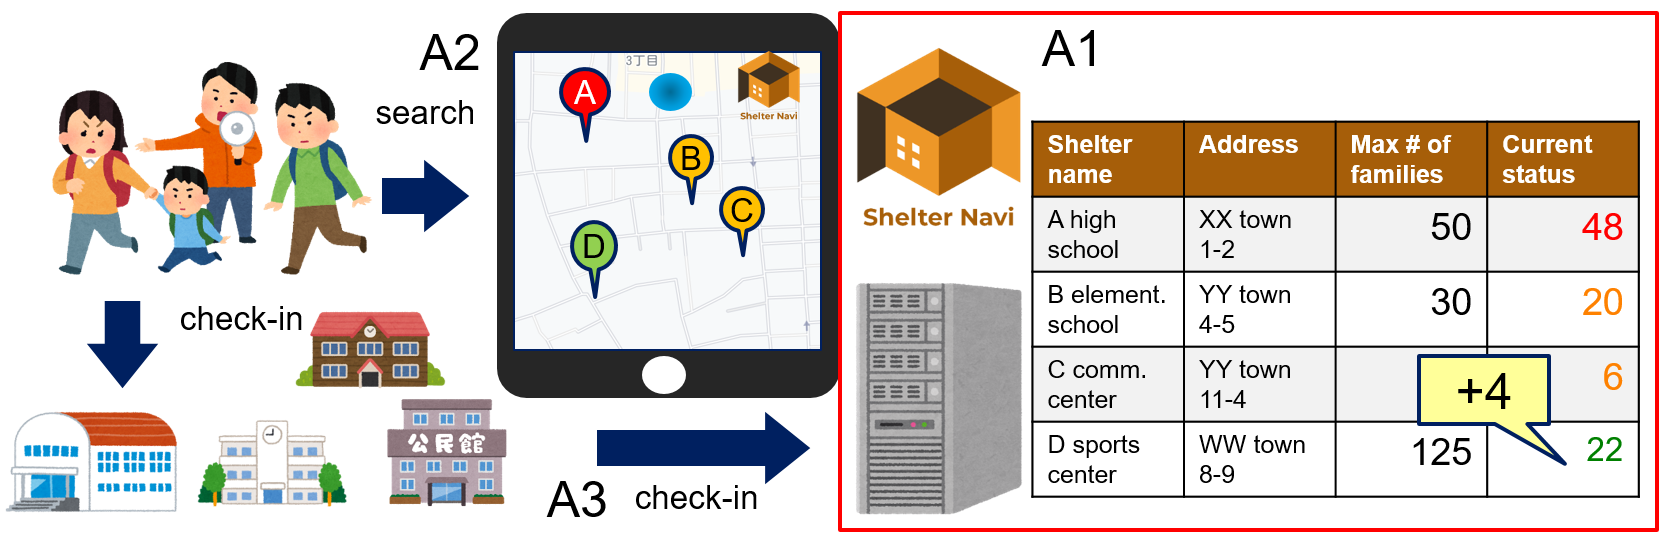
\includegraphics[scale=0.6,pagebox=cropbox,clip]{img/system.png}
          \caption{ShelterNaviの全体概要図}
          \label{fig:system}
     \end{center}
\end{figure*}

\begin{description}
     \item[A1.] クラウドサーバによる避難所の情報の管理
     
     Shelter Naviは,自治体が管理する避難所の情報をクラウドサーバで管理する.避難所の情報はマスタ情報と状態情報に分かれる.マスタ情報は,避難所名,住所,緯度経度,収容可能人数,管理人等で構成され,事前に自治体の職員によって登録されるものとする.状態情報は,各避難所の現在の収容者,収容人数,混雑度合い等で構成され,A3で後述するチェックインによって更新される.また,Shelter Naviを利用する住民は,住民ユーザ情報をクラウドサーバに登録する必要がある.住民ユーザ情報は氏名,メールアドレス,パスワード,世帯人数,自宅住所である.

     \item[A2.] リアルタイムな避難所混雑状況の配信と可視化
     
     災害が発生した際,Shelter NaviはA1の避難所情報を地図上に可視化する.住民は自身のスマートフォンで,自分の現在地(GPSで取得)と近隣の避難所(地図上のピンで表示)を確認する.各避難所の混雑度は,ピンの色や詳細情報で確認できるため,住民は自身の状況と混雑状況に基づいて,最適な避難所を自分で探し避難を行う.

     \item[A3.] 避難所へのチェックイン
     
     目的の避難所に到着したら,住民はスマートフォンのアプリケーション上でチェックイン操作を行う.Shelter Naviはその住民のチェックイン時刻をクラウドサーバに記録するとともに,住民の世帯人数をその避難所の収容人数に加算し,混雑状況を更新する.チェックイン機能により,各避難所に収容されている住民とその数を職員の手を借りずに自動集計できる.また,スマートフォンの扱いに不慣れな住民のために,担当者が住民のチェックインを代理で行う機能も提供する.
\end{description}

\subsection{ユースケース}
Shelter Naviで実現する機能を明確化するために,ユースケース定義を行う.Shelter Naviの利用者は,住民と自治体職員であり,それぞれのユーザロールでユースケース定義を行う.なお,住民のユーザ登録は住民自身が行うが,自治体職員のユーザ登録はShelter Naviの管理者が行うものとする.これは,自治体職員ユーザが災害時に住民の個人情報を参照するためであり,セキュリティ上の考慮である.図\ref{fig:usecase}にShelter Naviのユースケース図を示す.


\begin{figure}[!t]
     \begin{center}
          
\includegraphics[scale=0.35,pagebox=cropbox,clip]{img/usecase.png}
          \caption{ユースケース図}
          \label{fig:usecase}
     \end{center}
\end{figure}


\subsubsection{住民ユースケース}
住民のユースケースとして,以下のC1~C3を示す.
\begin{description}
     \item[C1.] 住民情報を登録する
     
     住民はShelter Naviの利用にあたり,事前に自身の住民情報を登録する必要がある.サインアップ画面から,氏名,メールアドレス,パスワード,世帯人数,住所などの情報を登録する.登録後,住民はメールアドレスとパスワードでアプリにログインする.

     \item[C2.] 避難所を検索する
     災害発生時に,住民は近隣の避難所をShelter Navi上で検索する.自分の現在位置周辺の避難所が地図上にピンで表示され,その混雑度をピンの色で確認できる.また,ピンをクリックすると,その避難所の詳細情報を確認できる.詳細情報は,避難所名,住所等のマスタ情報と現在の混雑度等の状態情報である.

     \item[C3.] チェックインする
     住民は,目的の避難所に到着したら,Shelter Navi上でチェックイン操作を行う.システムは,その住民のチェックインを記録する.さらにシステムは,その避難所の収容人数にその住民の世帯人数を加算し,避難所の混雑状態を更新する.
\end{description}


\begin{figure*}[!t]
     \begin{center}
          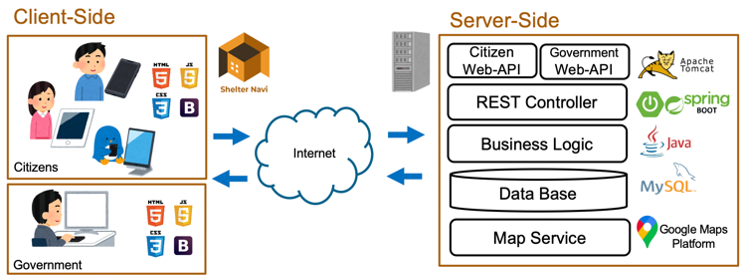
\includegraphics[width=0.8\linewidth,pagebox=cropbox,clip]{img/architecture.png}
          \caption{システムアーキテクチャ}
          \label{fig:architecture}
     \end{center}
\end{figure*}


\subsubsection{自治体ユースケース}
自治体ユースケースとして、以下のG1~G3を示す.

\begin{description}
     \item[G1.] 避難所を登録する
     自治体の担当職員が,避難所のマスタ情報を登録する.避難所名,住所,緯度経度,収容可能人数などのデータ項目を登録する.

     \item[G2.] 避難所の状態を確認する
     災害が発生した際,自治体の担当職員が各避難所の状態を確認する.画面には,地域内の全自治体のリストと混雑r状況がリアルタイムに表示される.特定の避難所を選択することで,チェックインしている住民の情報や人数を確認できる.これにより,自治体職員は混雑状況確認のために避難所に直接赴く必要がなくなり,感染拡大防止及び職務負担軽減につながる.

     \item[G3.] 住民の安否確認をする
     災害時に,自治体の担当職員が,特定の住民の安否確認を行うことができる.名前やメールアドレスで住民を検索し,どの避難所に避難しているか,いつチェックインしたか等の情報を確認する.安否確認は,親族や病院等,関係者や関係機関からの要請に基づいて,自治体職員が行うことを想定している.
\end{description}

\subsection{システムアーキテクチャ}

図\ref{fig:architecture}にShelter Naviのシステムアーキテクチャのイメージを示す.Shelter Naviはクライアント・サーバ方式のWebアプリケーションとして構成される.

サーバサイドは,クラウドサーバの機能を配置し,避難所,ユーザ,チェックイン等の主要なデータを管理する.コントローラ層,ドメイン層,永続層を有する典型的なレイヤードアーキテクチャを採用し,データや操作へのアクセスは,REST-APIを通して行う.また,地図機能のために,外部の地図クラウドサービスを連携して利用する.サーバサイドで利用する技術としては,Javaを実装言語とし,Spring Bootアプリケーションフレームワーク,Apache Tomcat Webサーバを用いる.また,データベースはMySQL,地図サービスにはGoogle Maps APIを用いる.

一方クライアントサイドには,主にユーザインタフェースの機能を配置する.OSや機種の違いを意識せずに済むように,スマートフォンまたはPCのWebブラウザ上でShelter Naviのユースケースを実行できるようにする.HTML,CSS,JavaScriptを実装言語とする.また,スマートフォンの画面で使いやすいように,Bootstrapを利用したレスポンシブルデザインを取り入れる.



\subsection{ドメインモデリング}

\subsubsection{全体の構成とエンティティ関連}

Shelter Naviで管理する情報を明確化するために,ドメインモデリングを行う.
図\ref{fig:domain}にShelterNaviのドメインモデル図を示す.
図\ref{fig:domain}に示すように,Shelter Naviのドメインには5つのエンティティが存在し,それぞれShelter(避難所),User(住民・ユーザ),Check-In(避難所へのチェックインまたはチェックアウト),ShelterState(避難所の状態),UserState(ユーザの状態)となっている.

Check-Inは,あるユーザとそのユーザが利用した避難所を関連付けるもので,1回のCheck-Inには必ず1つのUserと1つのShelterが結びつく.また,ShelterStateは各避難所の状態を表しており,UserStateはユーザの避難状態を示している.それぞれ,新しいCheck-Inオブジェクトが生成された際に,更新・作成される.
以下では,ShelterNaviの各エンティティのデータ項目を説明する.

\begin{figure}[!t]
     \begin{center}
          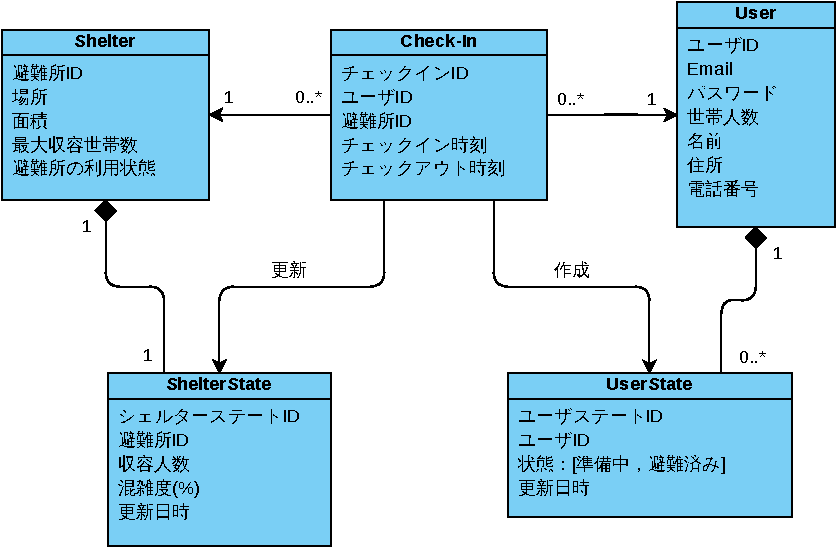
\includegraphics[width=\linewidth,pagebox=cropbox,clip]{img/domain_model.pdf}
          \caption{ドメインモデル図}
          \label{fig:domain}
     \end{center}
\end{figure}

\subsubsection{{\bf Shelter:} 避難所エンティティ}

Shelterエンティティは,システムがどの避難所かを識別するためのIDを持っている.また,避難するユーザに向けて避難所の名称,位置情報を示す必要がある.そして,避難所の開放情報も取り扱う.
%以上のことからShelterエンティティは以下のスキーマを規定する.

\begin{itemize}
    \item{\textbf{sid:}}避難所ID
    \item{\textbf{name:}}避難所の名称
    \item{\textbf{address:}}避難所の住所
    \item{\textbf{lat:}}避難所の緯度
    \item{\textbf{lng:}}避難所の経度
    \item{\textbf{capacity:}}避難所の収容可能人数
    \item{\textbf{isActive:}}避難所が利用可能か
\end{itemize}

\subsubsection{{\bf User:} ユーザエンティティ}
Userエンティティは,ユーザを一意に識別するユーザIDが必要である.また,本サービスに登録するためのemailアドレスとパスワード,安否確認で必要となる名前,住所,混雑度を計算するための世帯人数を取り扱う.% 本アプリにおける名前,住所,電話番号の必要性
%以上のことからUserドメインでは以下のスキーマを規定する.

\begin{itemize}
    \item{\textbf{uid:}}ユーザID
    \item{\textbf{email:}}メールアドレス
    \item{\textbf{password:}}パスワード
    \item{\textbf{name:}}ユーザの名前
    \item{\textbf{address:}}ユーザの住所
    \item{\textbf{of families:}}世帯人数
\end{itemize}

\subsubsection{{\bf Check-In:} チェックインエンティティ}
Check-Inエンティティは,どのユーザがどの避難所にチェックインしたかを管理するために,ユーザIDと避難所IDが必要である.また,複数の避難所への多重チェックインがないかを確認するために,チェックイン時刻と,チェックアウト時刻も取り扱う.%以上のことからCheck-Inドメインでは以下のスキーマを規定する.

\begin{itemize}
    \item{\textbf{cid:}}チェックインID
    \item{\textbf{uid:}}ユーザID
    \item{\textbf{sid:}}避難所ID
    \item{\textbf{checkin-datetime:}}チェックイン時刻
    \item{\textbf{checkout-datetime:}}チェックアウト時刻
\end{itemize}

\subsubsection{{\bf ShelterState:} 避難所の状態}
ShelterStateエンティティは,住民のチェックイン(およびチェックアウト)とともに変化する避難所の状態を表現する.対象とする避難所のID,現在の収容人数,現在の混雑度,更新日時を属性として持つ.収容人数は,現在チェックインしている全てのユーザの世帯人数の合計から算出する.また,混雑度は,収容人数を避難所の収容可能人数で割ることで求める.
%以上のことからShelterStateドメインでは以下のスキーマを規定する.

% 現在の収容人数のスキーマ名なににするべきか...
\begin{itemize}
     \item{\textbf{id:}}避難所の状態ID
     \item{\textbf{sid:}}避難所ID
     \item{\textbf{num of people:}}収容人数
     \item{\textbf{congestion:}}混雑度
     \item{\textbf{changedAt:}}更新日時
 \end{itemize}

\subsubsection{{\bf UserState:} ユーザの状態}
UserStateエンティティは,ユーザの避難状態とその履歴を管理する.特定のユーザの履歴を見るためにユーザIDが必要である.そして,在宅,準備中,避難中,避難済の避難状態を表す.また,避難状態が変化した際の日時を記録する.なお,ユーザの状態は履歴データを参照できるように,1つのデータを更新していくのではなく,新規データを追加していく形をとる.

\begin{itemize}
     \item{\textbf{id:}}ユーザの状態ID
     \item{\textbf{uid:}}ユーザID
     \item{\textbf{state:}}避難状態[在宅, 準備中, 避難中, 避難済]
     \item{\textbf{changedAt:}}更新日時
\end{itemize}


% CitizenStateドメインではユーザの状態しか取り扱わない?
% Citizenドメインのフィールドとするのはダメなのかチェックする

\subsection{主要なサービス}
\label{sec:service}
ドメインモデルの各エンティティを操作する主要なサービスを設計する.
ShelterNaviでは他のアプリケーションとの連携や拡張性を考慮し,HTTP-RESTによって呼び出し可能なRESTful Web-APIとして配備した.以下に各サービスの詳細を示す.

\subsubsection{{\bf ShelterService:} 避難所サービス}
避難所のCRUD(生成,読出,更新,削除)を行うサービスである.以下にAPIの一覧を示す.
\begin{itemize}
    \item{\textbf{createShelter( shelterForm ):}
         避難所ID,避難所名,位置情報を基に避難所データを作成し,取得する.}
    \item{\textbf{getShelter( sid ):}
         避難所IDを指定することで該当する避難所データを取得する.}
    \item{\textbf{deleteShelter( sid ):}
         避難所IDを指定することで該当する避難所データを削除する.}
    \item{\textbf{clearAllShelters():}
         全ての避難所データを削除する.}
    \item{\textbf{getAllShelters():}
         全ての避難所データを取得する.}
    \item{\textbf{searchSheltersByDistance( lng, lat, distance ):}
         経度,緯度,そして距離を指定することで,指定位置座標(lng, lat)から半径distance$\rm[km]$以内にある避難所データ全てを取得する.当APIでは,地球上における大圏距離を計算する手法を採用し,ユーザの現在位置$p$と与えられた避難所の距離$s$の間の直線距離$d(p,s)$計算する.具体的には,地球の半径を6371[km],ユーザの経度座標を$lng$,緯度座標を$lat$,各避難所データの経度座標を$s.lng$,緯度座標を$s.lat$としたとき,$d(p,s)$を以下の計算式で求める.
         \begin{eqnarray*}
          &d(&p,s) = 6371 \times \arccos (\\
          & &\cos( rad(lat ) ) \times \cos( rad( s.lat ) ) 
          \times \cos( rad( s.lng ) - rad(lng ) ) \\
          & & +  \sin( rad( lat ) ) \times \sin( rad( s.lat ))\\
          &)&
         \end{eqnarray*}}
    \item{\textbf{searchSheltersByKeyword( keyword ):}
         文字列を指定して避難所を検索する.避難所名,または避難所住所に部分一致する避難所エンティティを全て取得する.}
\end{itemize}

\subsubsection{{\bf UserService:} ユーザサービス}
ユーザのCRUDを行うサービスである.以下にAPIの一覧を示す.
\begin{itemize}
    \item{\textbf{createUser( userForm ):}
         メールアドレス,パスワード,名前,住所,世帯人数を含むユーザ情報を元に新規ユーザを作成する.}
    \item{\textbf{getUser( uid ):}
         ユーザIDを指定することで該当するユーザエンティティを取得する.}
    \item{\textbf{updateUser(uid, userForm ):}
         ユーザフォームを入力して,既存のユーザ情報を更新する.}
    \item{\textbf{deleteUser( uid ):}
         ユーザIDを指定することで該当するユーザエンティティを削除する.}
\end{itemize}

\subsubsection{{\bf CheckInService:} チェックインサービス}
避難所へのチェックイン,チェックアウト操作を行うサービスである.
以下にAPIの一覧を示す.
\begin{itemize}
    \item{\textbf{checkIn( uid, sid ):}
         ユーザIDと避難所IDを指定して,チェックイン処理を行う.具体的には,Check-Inオブジェクトを新規作成し,作成日時を記録する.同時に,避難所の収容人数をそのユーザの世帯人数分増加させ,避難所の混雑度を再計算して,ShelterStateオブジェクトを更新する.さらに,避難状態を「避難済」に設定したUserStateオブジェクトを新規作成する.}
    \item{\textbf{checkOut( uid, sid ):}
         ユーザIDと避難所IDを指定して,チェックアウト処理を行う.
         ユーザIDと避難所IDから一意に定まる最新のチェックインデータを取得し,チェックアウト時刻を記入する.同時に,避難所の収容人数をそのユーザの世帯人数分減少させ,避難所の混雑度を再計算して,ShelterStateオブジェクトを更新する.さらに,避難状態を「避難中」に設定したUserStateオブジェクトを新規作成する.}
\end{itemize}

%% ↓ これらはチェックインサービスから内部的に呼び出されるものとして修正した.
%\subsubsection{シェルターステートサービス}
%\begin{itemize}
%     \item{\textbf{checkIn( uid, sid ):}
%          ユーザIDと避難所IDを指定することで,避難所の収容人数をユーザの世帯人数分増加させ,避難所の混雑度を計算し,更新する.また,更新日時を記録する.}
%     \item{\textbf{checkOut( uid, sid ):}
%          ユーザIDと避難所IDを指定することで,避難所の収容人数をユーザの世帯人数分減少させ,避難所の混雑度を計算し,更新する.また,更新日時を記録する.}
%\end{itemize}

%\subsubsection{ユーザステートサービス}
%\begin{itemize}
%     \item{\textbf{checkIn( uid ):}
%          ユーザIDを指定することで,特定のユーザの避難状態を「避難済み」にしたUserStateのデータを新規で作成する.また,更新日時も併せて記録する.}
%     \item{\textbf{checkOut( uid ):}
%          ユーザIDを指定することで,特定のユーザの避難状態を「準備中」にしたUserStateのデータを新規で作成する.また,更新日時も併せて記録する.}
%\end{itemize}

\section{実装}
\subsection{Shelter Naviプロトタイプの実装}
前述した設計に基づき,Shelter Naviのプロトタイプを実装した.
今回のプロトタイプでは,住民ユースケースC1~C3をカバーする.
避難所のデータは神戸市の指定緊急避難所335件,姫路市の指定避難所255件をデータベースに手動で登録した.これらの避難所データは,神戸市\cite{kobe_open_data}および姫路市\cite{himeji_open_data}が公開する避難所オープンデータに基づいて作成した.

プロトタイプ実装で用いた技術は以下のとおりである.
\begin{itemize}
    \item サーバ開発言語:Java
    \item アプリケーションフレームワーク:Spring Boot
    \item データベース:MySQL 8.0.20
    \item Webサーバ:Apache Tomcat 9.0
    \item クライアント開発言語:HTML5, JavaScript
    \item CSSライブラリ:Bootstrap 4
\end{itemize}

以下ではShelterNaviの「ログイン」,「サインアップ」,「避難所検索」,「チェックイン」の各画面を例に挙げて,作成したプロトタイプ実装を概説する.


\subsection{ログイン}


Shelter Naviのログイン画面を図\ref{fig:login}に示す.
住民ユーザは画面中央のフォームにメールアドレスとパスワードを入力してログインする.正しいメールアドレスとパスワードが入力できていれば,認証が成功し避難所検索画面に移行する.認証が成功すると,そのユーザに関連するエンティティにアクセスの認可が許可される.一般住民ユーザに認可・付与される権限では,自身のエンティティへのアクセスしか認可されないため,自分の情報が他ユーザから閲覧,更新,削除されることはない.

ユーザ情報をまだ登録していない場合には,「新規登録」ボタンを押すことで,次節で述べるサインアップ画面に移行する.

\begin{figure}[t]
     \begin{center}
          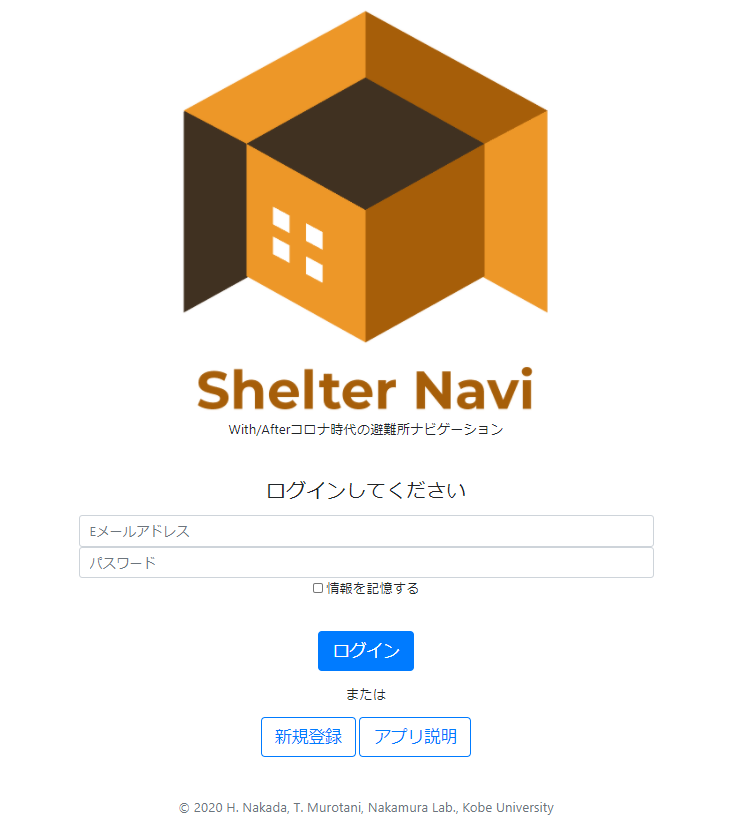
\includegraphics[scale=0.5,pagebox=cropbox,clip]{img/login.png}
          \caption{ログイン画面}
          \label{fig:login}
     \end{center}
\end{figure}

%今回の実装においては,セキュリティ性を担保するためにJavaのフレームワークであるSpring Securityを用いる.このフレームワークの機能を利用すれば,指定したURL内で,IDとパスワードをPostする特定のAPIを利用することで認証が可能になる.また,ユーザオブジェクトに権限を付与し,その権限に応じた認可を与えることも可能になる.本アプリケーションでは,通常の工程でユーザを作成した場合,CITIZEN(住民・一般ユーザ)の役割が付与される.実際には,ログイン機能における認証時にこの役割を見ることで,セッションに対して役割に対応した権限を付与する.これによりログイン後のユーザに対する各ページへの認可が可能になる.

\subsection{サインアップ}
\label{sec:signup}
サインアップ画面を図\ref{fig:signup}に示す.
住民が自身のユーザ情報をフォームに入力し,新規登録を行う.ユーザの識別に必要なメールアドレスと,認証に必要なパスワードを指定する.また,システム内で扱われる名前,住所,世帯人数,電話番号(任意)からなる「個人情報」も併せて入力する.これらの情報を入力したうえで図\ref{fig:signup}下部の登録ボタンをクリックすれば,ユーザ新規登録の完了となる.

\begin{figure}[t]
     \begin{center}
          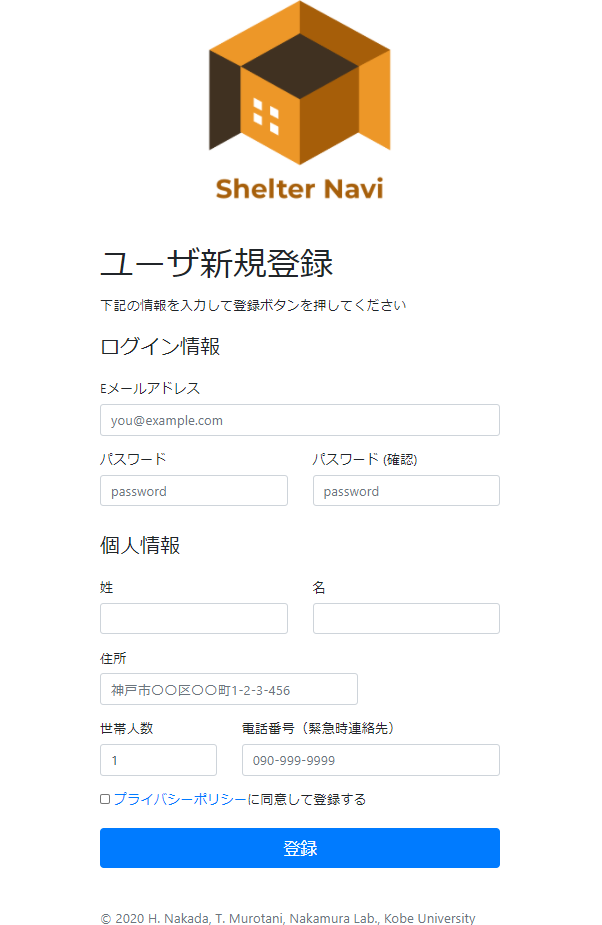
\includegraphics[scale=0.6,pagebox=cropbox,clip]{img/signup.png}
          \caption{サインアップ画面}
          \label{fig:signup}
     \end{center}
\end{figure}

\subsection{避難所検索}
避難所検索画面を図\ref{fig:search_shelter}に示す.

\begin{figure}[t]
     \begin{center}
          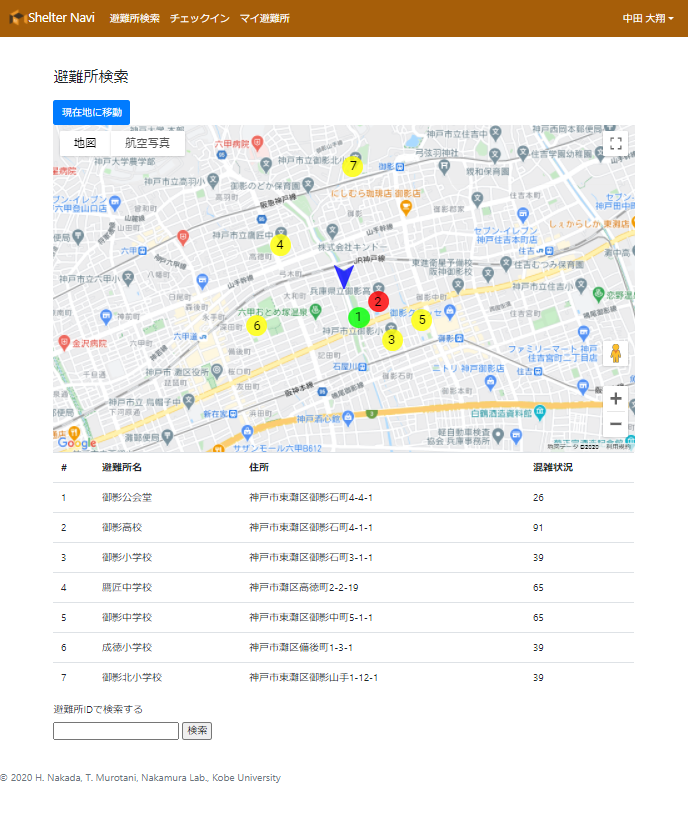
\includegraphics[scale=0.6,pagebox=cropbox,clip]{img/search_shelter.png}
          \caption{避難所検索画面}
          \label{fig:search_shelter}
     \end{center}
\end{figure}

避難所検索画面では画面上部に青いマーカーを現在地とした地図が表示される.地図上には,現在地周辺(プロトタイプでは半径1$\rm[km]$以内としている)の避難所を番号付きのピンで配置している.
周辺の避難所の検索は\ref{sec:service}で紹介したAPI,searchSheltersByDistance()を利用してリアルタイムで更新する.
ピンの色は,避難所の混雑度の値に応じて,緑(低い),黄色(中程度),赤(高い)の色で表示される.避難所のピンをクリックすることで避難所の詳細情報を表示することもできる.

画面下部のリストには,地図上の避難所が距離が近い順に表示される.リストの各項目は,左から地図上のマーカーの番号,避難所名,避難所の住所,混雑状況の4つである.最後に,画面最下部に検索バーでは,避難所ID,名称,住所で避難所を検索できる.

%実際は管理者が直接データを入れることになりそうなので機能ではない?

\subsection{チェックイン}
チェックイン画面を図\ref{fig:checkin}に示す.チェックイン画面では,チェックインする避難所を「現在地」,「エリア」,「地図」のいずれかから選択することができる.「現在地」から選択する場合,画面上部の青色の「現在地を取得」ボタンをクリックすれば,現在地に存在する避難所を選択することができる.「エリア」から選択する場合は,画面中央の「エリアから選択」の項目である都道府県,市町村,地域をプルダウンメニューから選択することで避難所のプルダウンメニューに条件に該当する避難所リストが現れる.「地図」から選択する場合は,画面下部の地図上にある赤いマーカーをクリックすることで避難所の選択が可能になる.これらのいずれかの方法で避難所を選択してから画面右下の「チェックインする」ボタンを押すことで避難所へのチェックインが完了する.
%本アプリケーションでは,避難所を可視化する上でGoogle Mapを利用している.避難所を取得するAPIで避難所データを取得し,それらのデータをGoogleMapsAPIで利用することで,地図上への避難所の可視化を行っている.また,ShelterNaviではユーザの現在位置に応じて地図上に表示する避難所を変更しており,これは「3.5 主要なサービス」で言及したsearchSheltersByDistance(lng, lat, distance)をを利用している.

%\subsection{チェックアウト}
チェックアウト画面を図\ref{fig:checkout}に示す.
いずれかの避難所にチェックイン済みの場合,チェックアウト画面左下には「現在の避難所:「※チェックイン済みの避難所名」からチェックアウトしますか?」の1文が表示される.画面右下の「チェックアウトする」ボタンを押すことで,現在チェックインしている避難所からのチェックアウトが完了する.

\begin{figure}[t]
     \begin{center}
          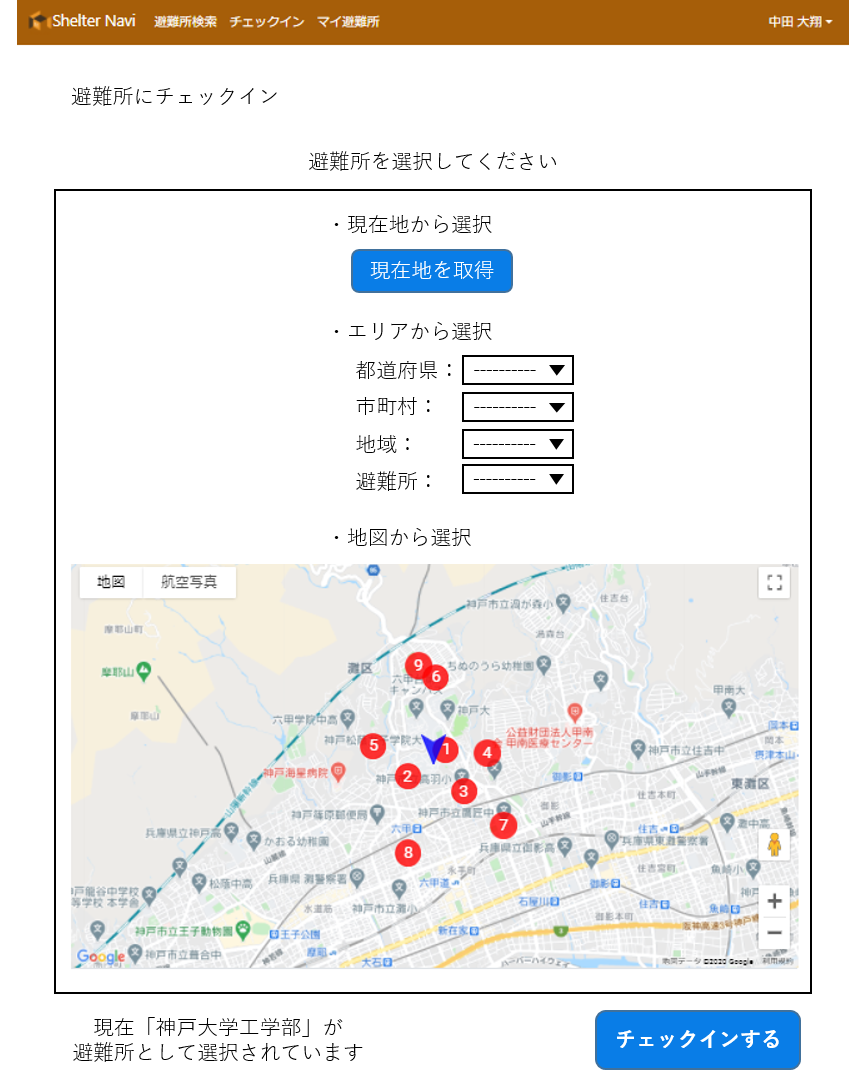
\includegraphics[scale=0.6,pagebox=cropbox,clip]{img/checkin.png}
          \caption{チェックイン画面}
          \label{fig:checkin}
     \end{center}
\end{figure}

\begin{figure}[t]
     \begin{center}
          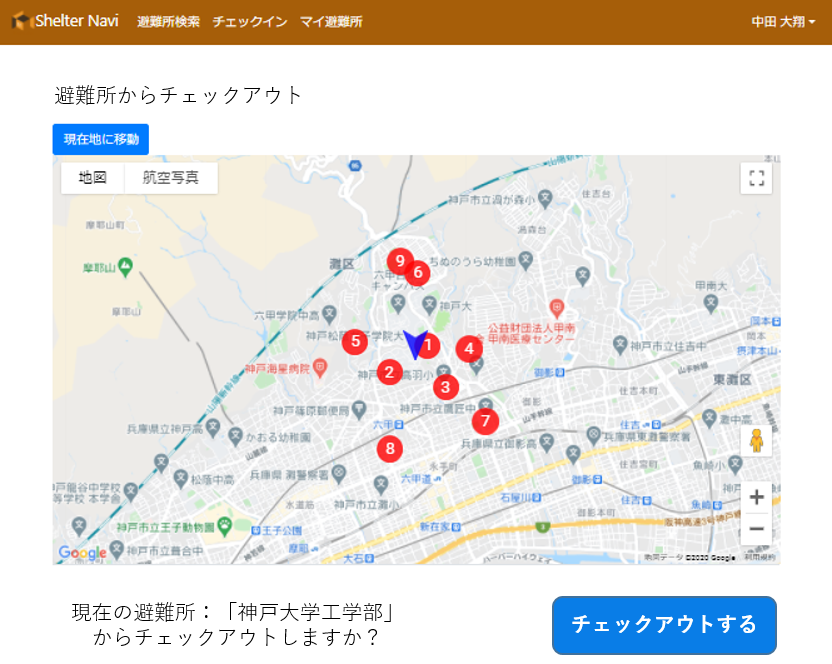
\includegraphics[scale=0.6,pagebox=cropbox,clip]{img/checkout.png}
          \caption{チェックアウト画面}
          \label{fig:checkout}
     \end{center}
\end{figure}

\section{考察}
\subsection{ShelterNaviの効果・メリット}
Shelter Naviの実現によって得られる効果・メリットとして,以下の3点が挙げられる.

1つ目は,住民が受け入れ人数に余裕のある避難所を自力で見つけることができる点である.これは,本稿のリサーチクエスチョンである「住民が自治体に頼ることなく,自分たちで適切な避難所へ分散避難できないか?」という課題の解決に資するものである.

2つ目は,避難所の混雑度が住民のチェックインとシステムによって自動的に算出・更新される点である.これによって,各避難所に混雑状況を管理する専任職員を置く必要がなくなる.

3つ目は,自治体の職員がリアルタイムで登録されている全避難所の状況を確認できる点である.各避難所の状況をShelter Naviで一括横断的に管理できるため,自治体職員の職務負担を軽減するとともに,安否確認や分散避難指示など,従来では困難だった避難所運営のアクションが可能となる.

\subsection{ShelterNaviの限界}
我々が現状で把握しているShelter Naviの限界として,以下の3つが挙げられる.

1つ目は,正確な避難所情報の登録が必要となる点である.具体的には,平時において避難所の緯度経度や収容可能人数,開設状況等のマスタ情報を登録・保守する必要があり,これには自治体の協力が必須である.

2つ目は,スマートフォンの操作に慣れていない人にとって,Shelter Naviをうまく操作できるかという懸念である. Shelter Naviはスマートフォンでの使用を前提としたアプリケーションであるため,スマートフォンの操作に不慣れな,またスマートフォンを所有していない高齢者などの人々にとって,このアプリケーションを利用することは難しいと予想される.

3つ目は,アプリケーションがモバイル通信網に依存しているという点である.災害時にモバイル通信網が不通になった場合,サーバへアクセスできなくなるため,Shelter Naviが動作しない.

\section{おわりに}

本研究ではコロナ時代の災害を想定し,住民の自助によって避難所での密の形成を回避し,迅速且つ安全な避難の実現を支援するモバイル・アプリケーション Shelter Navi を提案した.
クラウドサーバによる避難所の混雑状態の管理・可視化と,住民による避難所の検索とチェックインによって,各避難所に特別な設備を必要とすることなく,避難所での密を考慮した避難が可能となる.
また,Shelter Navi のユースケース定義,ドメインモデル,サービスの設計を行い,プロトタイプをWebアプリケーションとして実装した.

今後の課題としては,実際の避難を想定した有効性評価を行うことである.
これには,近隣の自治体に協力を依頼して避難所データの整備を行ったうえで,避難訓練等の機会に住民に試用・評価してもらうことを考えていきたい.
また,Shelter Naviの機能強化も併せて行う予定である.
まずはユーザによる私的な避難所(親類宅や友人宅など)の登録・管理機能の追加があげられる.
さらには,避難所での情報共有や避難者同士のコミュニケーション等,チェックイン後の避難生活の質を向上する機能も考えていきたい.

\ack %% 謝辞
本研究は,
JSTグローバルサイエンスキャンパス ROOTプログラム,
JSPS科研費 JP19H01138, JP18H03242, JP18H03342, JP19H04154, JP19K02973,JP20K11059, JP20H04014, JP20H05706 の研究助成を受けて行われている.

%\bibliographystyle{sieicej}
%\bibliography{myrefs}
\begin{thebibliography}{99}% 文献数が10未満の時 {9}
\bibitem{1} 国土交通省 “平成30年7月豪雨災害の概要と被害の特徴”
\bibitem{2} 菊池聡, “非常時の思い違いと批判的思考” 日本科学教育学会年会論文集, Vol.35, pp.9-10, 2011.
\bibitem{3} 国土交通省 “住民自らの行動に結びつく災害情報の提供へ ~危機感が伝わる、メディアとの連携策をとりまとめ~” 2018.12.11
\bibitem{4} 皆川勝、中村遼太、高橋翔天 “極低頻度の災害に対する避難行動の社会心理学的な考察” 土木学会論文集F6 Vol.72 No.2 I191~I198 2015.7.10
\bibitem{5} 田中重好 “東日本大震災を踏まえた防災パラダイム転換” Vol.64 No.3 p.342-365 2013.
\bibitem{6} 内閣府 “新型コロナウイルス感染症を踏まえた災害対応のポイント【第1版】について”
\bibitem{7} 毎日新聞 “避難所「先着順で満員、2回も振られる」台風10号、コロナ対策で収容人数の減少で” 2020.09.07
\bibitem{8} 株式会社バカン “株式会社バカンと宮崎県日南市、災害発生時にIoTを活用して避難所の混雑情報配信を支援する協定を締結” 2020.08.03
\bibitem{9} Spring “Why Spring?” https://spring.io/why-spring
\bibitem{kobe_open_data} 神戸市,‘‘災害時の避難所'', 
\url{https://www.city.kobe.lg.jp/a46152/bosai/prevention/evacuation.html}
\bibitem{himeji_open_data} 姫路市,``オープンデータカタログサイト'',
\url{https://city.himeji.gkan.jp/gkan/dataset/hinanshisetsu}

\end{thebibliography}

\end{document}

